\subsection{Монтировки телескопов}
Монтировки телескопов разделяют на два основных вида: \imp{экваториальная} и \imp{альтзимутальная} монтировка (см.~Рис.\,\ref{mounts}).
\begin{figure}[h]
	\centering
	\hspace*{.4cm}
	\begin{subfigure}{0.48\textwidth}
		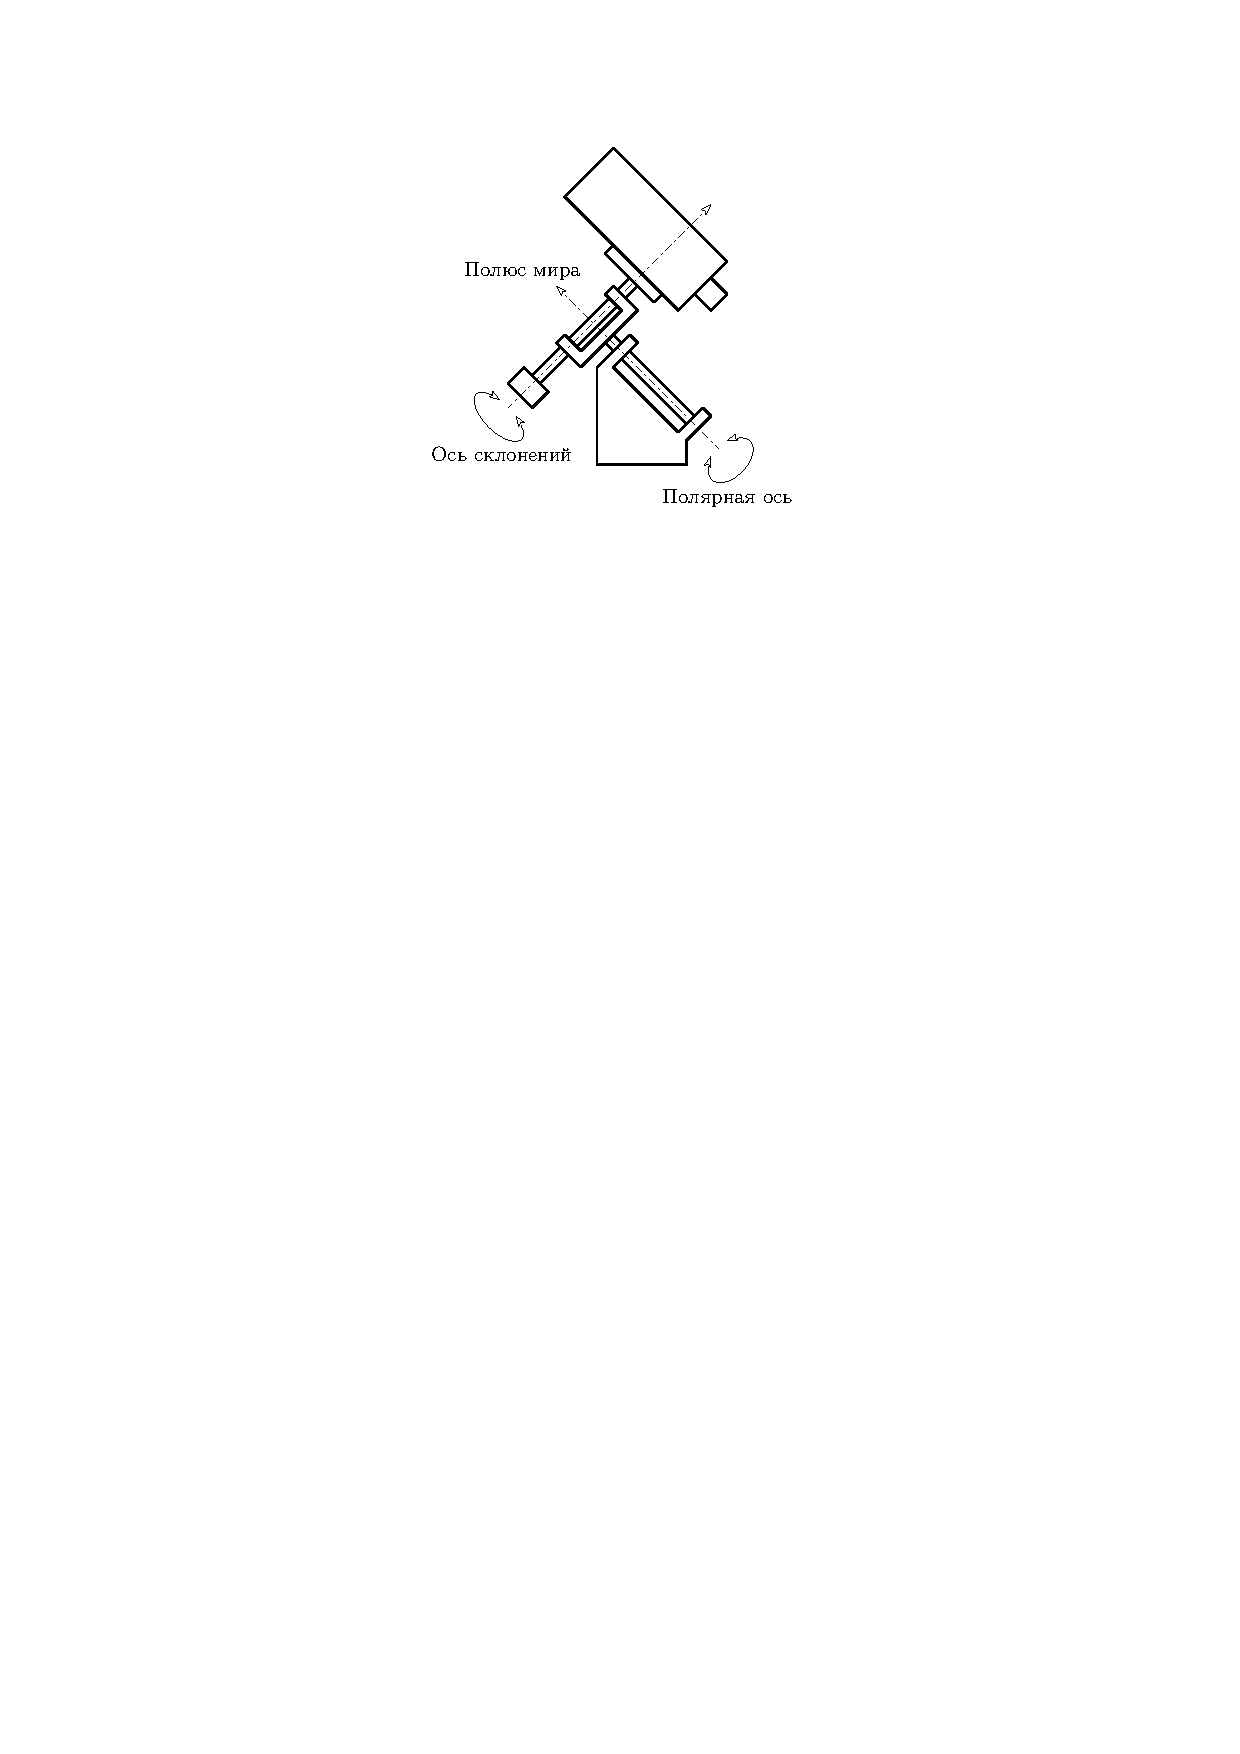
\includegraphics[height = 5cm]{mount-eq}
		\caption{Экваториальная мортировка}
	\end{subfigure}
	\hspace*{.4cm}
	\begin{subfigure}{0.41\textwidth}
		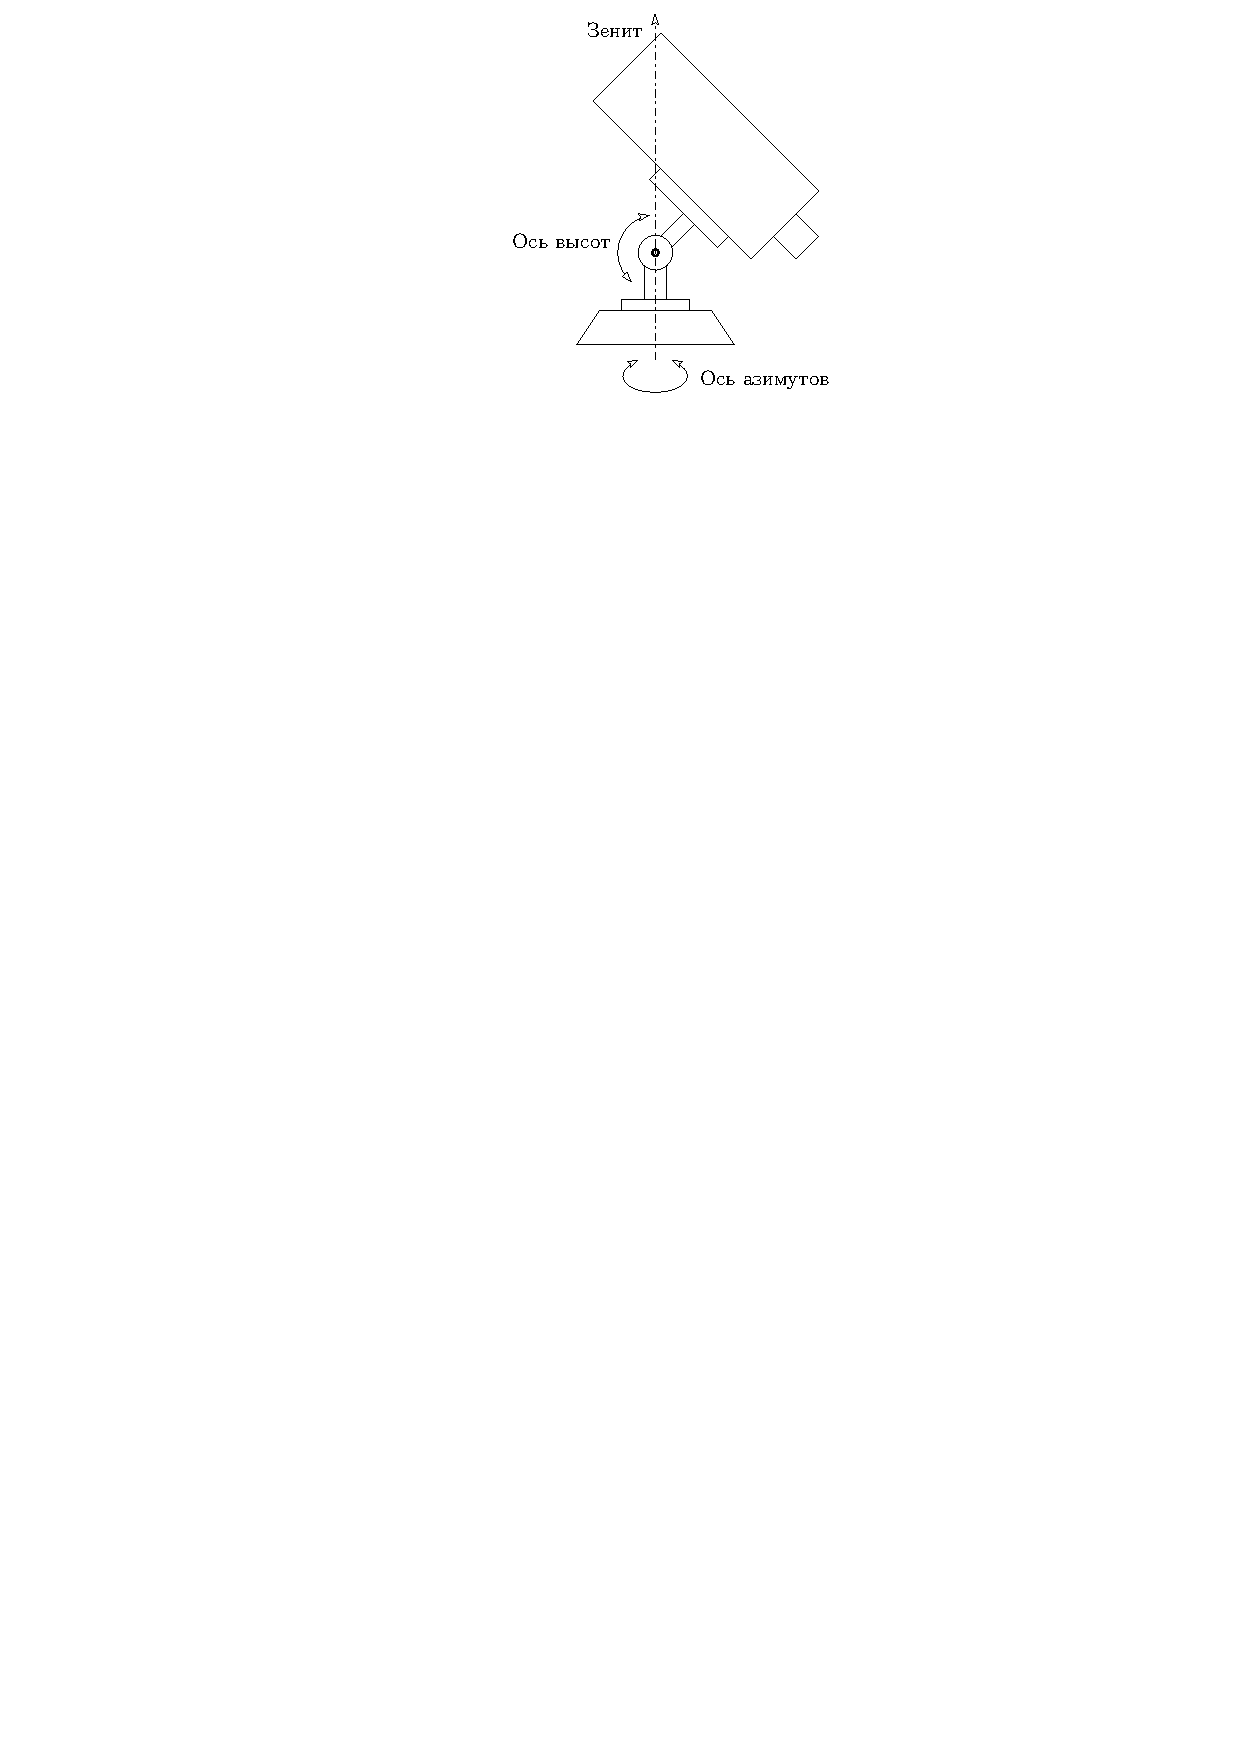
\includegraphics[height = 5cm]{mount-alt}
		\caption{Альтзимутальная монтировка}
	\end{subfigure}
	\hspace*{.4cm}
	\caption{Виды монтировок}
	\label{mounts}
\end{figure}

\term{Экваториальная монтировка}~--- монтировка, одна ось которой направлена на полюс мира (полярная ось), а другая параллельна небесному экватору (ось склонения).
Для гидирования на такой монтировке, нужно лишь поворачивать её с постоянной угловой скоростью вокруг полярной оси в направлении роста часового угла.
Важно отметить, что существует несколько разновидностей экваториальных монтировок: \imp{немецкая}, \imp{английская}, \imp{американская} монтировки и монтировка \imp{с рамой}.

\term{Альтзимутальная монтировка}~--- монтировка телескопа, имеющая вертикальную и горизонтальную оси вращения, позволяющая поворачивать телескоп по высоте и по азимуту. Для слежения за небесными объектами, перемещающиеся по небесной сфере вследствие суточного вращения Земли, телескоп нужно поворачивать одновременно вокруг обеих осей с разными переменными скоростями.